\documentclass[11pt,letterpaper]{article}
\usepackage[margin=0.85in]{geometry}
\usepackage{amsmath}
\usepackage{xcolor}
\usepackage{titlesec}
\usepackage{tabularx}
\usepackage{booktabs}
\usepackage{listings}
\usepackage{fancyhdr}
\usepackage[hidelinks]{hyperref}

\hypersetup{
    colorlinks=true,
    linkcolor=blue!70!black,
    urlcolor=blue!70!black,
    citecolor=blue!70!black,
    pdfauthor={Vincent Randal and Antigravity Assistant},
    pdftitle={Software Design Description and Code Review: Word of God Project}
}

% Code listing styling
\definecolor{codegreen}{rgb}{0.1,0.5,0.1}
\definecolor{codegray}{rgb}{0.5,0.5,0.5}
\definecolor{codepurple}{rgb}{0.58,0,0.82}
\definecolor{backcolour}{rgb}{0.97,0.98,0.99}

\lstdefinestyle{codebox}{
    backgroundcolor=\color{backcolour},
    commentstyle=\color{codegreen},
    keywordstyle=\color{blue!80!black}\bfseries,
    numberstyle=\tiny\color{codegray},
    stringstyle=\color{codepurple},
    basicstyle=\ttfamily\footnotesize,
    breakatwhitespace=false,
    breaklines=true,
    captionpos=b,
    keepspaces=true,
    numbers=left,
    numbersep=8pt,
    showspaces=false,
    showstringspaces=false,
    showtabs=false,
    tabsize=2,
    frame=single,
    rulecolor=\color{black!20}
}
\lstset{style=codebox}

% Page header/footer styling
\pagestyle{fancy}
\fancyhf{}
\fancyhead[L]{\small\scshape Word of God: Software Design Description}
\fancyhead[R]{\small\scshape September 2026}
\fancyfoot[C]{\thepage}
\renewcommand{\headrulewidth}{0.4pt}
\renewcommand{\footrulewidth}{0.4pt}

% Section styling
\titleformat{\section}{\large\bfseries\scshape\color{blue!70!black}}{}{0em}{}[\titlerule]
\titleformat{\subsection}{\normalsize\bfseries\color{black!90}}{}{0em}{}

\begin{document}

\begin{titlepage}
    \centering
    \vspace*{2cm}
    {\huge\bfseries Software Design Description\\[0.3em] \& Code Review Specification\par}
    \vspace{1cm}
    {\Large\itshape Engineering Architecture for Slicing, Indexing, and Cloud Streaming the 1769 King James Bible\par}
    \vspace{2cm}
    {\large\textbf{Author:} Vincent Randal\par}
    {\large\textbf{Technical Reviewer:} Antigravity Assistant\par}
    \vspace{1cm}
    {\large Repository: \href{https://github.com/vtrandal/WordofGod}{github.com/vtrandal/WordofGod}\par}
    \vspace{2cm}
    \vfill
    {\normalsize Project: \texttt{WordofGod} $\cdot$ September 2026\par}
\end{titlepage}

\tableofcontents
\newpage

\section{Executive Summary \& System Architecture}

\subsection{Project Scope and Objective}
The primary objective of the \textbf{Word of God} project is to transform an monolithic 1,437-page compilation of the King James Bible (1769 Authorized Version) into a modern, modular, and portable multi-volume digital library. 

The architecture addresses three fundamental software challenges:
\begin{enumerate}
    \item \textbf{Lossless Document Decomposition}: Extracting 66 canonical books into standalone PDF files with zero text overlap and zero distortion of typography.
    \item \textbf{Dual-Tier Indexing (Local vs. Cloud)}: Enabling instant navigation across volumes through both local inter-document filesystem links (\texttt{/GoToR}) and high-speed cloud-streamed endpoints (\texttt{/URI}).
    \item \textbf{Cross-Platform Mobile Portability}: Overcoming mobile operating system (iOS/iPadOS) sandbox restrictions and MIME type download traps to deliver on-the-fly PDF streaming.
\end{enumerate}

\subsection{Architectural Component Matrix}
The system consists of five distinct, production-verified solutions working in synergy:

\begin{table}[h!]
\centering
\small
\begin{tabularx}{\linewidth}{p{3.5cm} p{2.8cm} p{2.5cm} X}
\toprule
\textbf{Component} & \textbf{Source File} & \textbf{Output Artifact} & \textbf{Core Role} \\
\midrule
\textbf{A. PDF Slicer} & \texttt{split\_bible.py} & \texttt{./books/*.pdf} (67) & Automated bookmark extraction and boundary page slicing. \\
\textbf{B. Local Master Index} & \texttt{Master\_Index.tex} & \texttt{Master\_Index.pdf} & Offline desktop navigation using relative PDF action links. \\
\textbf{C. Cloud Master Index} & \texttt{Master\_Index\_Cloud.tex} & \texttt{Master\_Index\_Cloud.pdf} & Mobile/iCloud streaming via high-speed GitHub CDN links. \\
\textbf{D. Web Bookshelf} & \texttt{index.html} & \texttt{index.html} & Zero-dependency responsive web portal with real-time search. \\
\textbf{E. Build Orchestrator} & \texttt{generate\_indexes.py} & Rebuilds B, C, D & Dynamic metadata aggregation and automated compilation. \\
\textbf{F. PWA Audio Reader} & \texttt{manifest.json, sw.js} & PWA Mobile App & Fullscreen mobile PWA with text reflow, synchronized verse audio, and offline caching. \\
\bottomrule
\end{tabularx}
\caption{System Component Architecture Overview}
\end{table}

\newpage
\section{Code Review: Solution A --- Automated Boundary Extraction}

\subsection{File: \texttt{split\_bible.py}}
\textbf{Purpose}: Decompose \texttt{KJV-Holy-Bible-1769.pdf} (1,437 pages) into 66 individual book PDFs plus one standalone front-matter PDF.

\begin{lstlisting}[language=Python]
import os, re
from pypdf import PdfReader, PdfWriter

PDF_PATH = "KJV-Holy-Bible-1769.pdf"
OUTPUT_DIR = "books"

def split_bible():
    os.makedirs(OUTPUT_DIR, exist_ok=True)
    reader = PdfReader(PDF_PATH)
    outline = reader.outline
    total_pages = len(reader.pages)

    # 1. Front Matter Extraction (Pages 0 to 3)
    first_book_page = reader.get_destination_page_number(outline[0])
    if first_book_page > 0:
        front_writer = PdfWriter()
        for p in range(first_book_page):
            front_writer.add_page(reader.pages[p])
        with open(os.path.join(OUTPUT_DIR, "00_Front_Matter.pdf"), "wb") as f:
            front_writer.write(f)

    # 2. Sequential Book Range Extraction (Books 1 to 66)
    for i, item in enumerate(outline):
        book_num = i + 1
        safe_title = re.sub(r"[^A-Za-z0-9_ -]", "", item.title).strip().replace(" ", "_")
        filename = f"{book_num:02d}_{safe_title}.pdf"

        start_page = reader.get_destination_page_number(item)
        end_page = reader.get_destination_page_number(outline[i + 1]) - 1 if (i + 1 < len(outline)) else (total_pages - 1)

        writer = PdfWriter()
        for p in range(start_page, end_page + 1):
            writer.add_page(reader.pages[p])

        with open(os.path.join(OUTPUT_DIR, filename), "wb") as f:
            writer.write(f)
\end{lstlisting}

\subsection{Design Analysis \& Engineering Decisions}
\begin{enumerate}
    \item \textbf{Outline Tree Traversal vs. OCR/Regex}: Instead of unreliable text-scraping across 1,437 pages, the algorithm reads the PDF document's native Outline Dictionary (\texttt{/Outlines}). Inspection revealed that the original LaTeX compilation cleanly contained exactly 66 top-level bookmarks.
    \item \textbf{Zero-Indexed Boundary Calculation}: In PDF specifications, page destinations are 0-indexed. The start page of book $i+1$ directly dictates the end page of book $i$ via:
    $$\text{end\_page}_i = \text{start\_page}_{i+1} - 1$$
    For the final volume (Revelation), the upper boundary clamps to $\text{total\_pages} - 1$.
    \item \textbf{Canonical Sorting Preservation}: Book filenames are prefixed with two-digit zero-padded numbers (\texttt{01\_Genesis.pdf} to \texttt{66\_Revelation.pdf}). This guarantees that operating systems and file managers list the books in canonical biblical sequence rather than alphabetical order.
\end{enumerate}

\newpage
\section{Code Review: Solution B --- Local Offline Master Directory}

\subsection{File: \texttt{Master\_Index.tex}}
\textbf{Purpose}: Provide a formal, 5-page master PDF that displays the original front matter and a two-column interactive directory linking to local files.

\begin{lstlisting}[language=TeX]
% Layout Architecture: Master_Index.tex
\documentclass[10pt,letterpaper]{article}
\usepackage[top=0.6in,bottom=0.6in,left=0.75in,right=0.75in]{geometry}
\usepackage{pdfpages}
\usepackage{tabularx}
\usepackage[hidelinks]{hyperref}

\begin{document}
% 1. Embed Original 4-page Front Matter
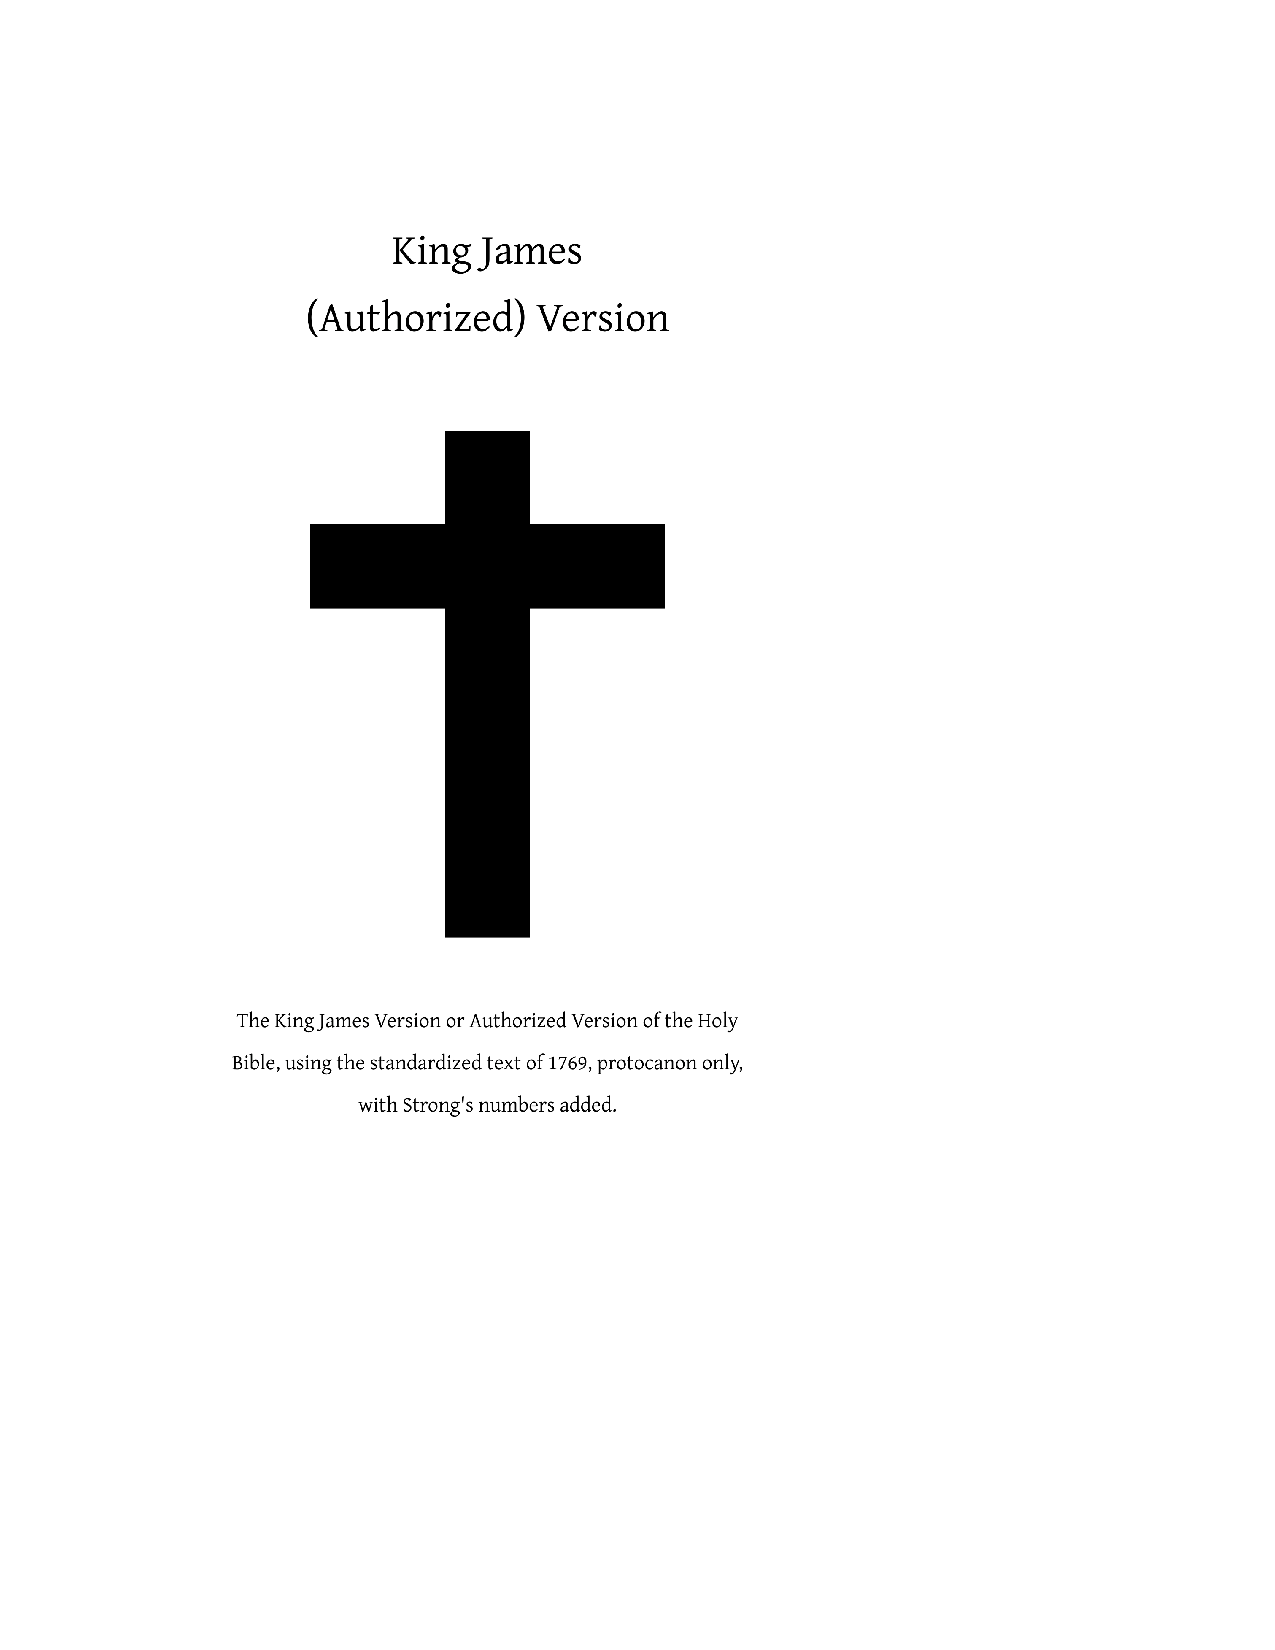
\includepdf[pages=-]{books/00_Front_Matter.pdf}

% 2. Page 5: Two-Column Single-Page Balanced Layout
\noindent
\begin{minipage}[t]{0.485\textwidth}
  \centering{\bfseries\scshape The Old Testament \footnotesize(39 Books)}\\
  \begin{tabularx}{\linewidth}{r X r}
    01 & \href{books/01_Genesis.pdf}{Genesis} & 68 pp. \\
    % ... books 2 through 39 ...
  \end{tabularx}
\end{minipage}\hfill
\begin{minipage}[t]{0.485\textwidth}
  \centering{\bfseries\scshape The New Testament \footnotesize(27 Books)}\\
  \begin{tabularx}{\linewidth}{r X r}
    40 & \href{books/40_Matthew.pdf}{Matthew} & 41 pp. \\
    % ... books 41 through 66 ...
  \end{tabularx}
\end{minipage}
\end{document}
\end{lstlisting}

\subsection{Design Analysis \& Engineering Decisions}
\begin{enumerate}
    \item \textbf{Layout Engineering (\texttt{minipage} vs. \texttt{multicols})}:
    Early iterations used the LaTeX \texttt{multicol} environment. However, because the Old Testament contains 39 rows and the New Testament contains 27 rows, \texttt{multicols} automatically attempted to balance column height, causing the Old Testament table to spill over onto Page 6. By refactoring the layout into two independent top-aligned \texttt{minipage} blocks with adjusted line spacing (\texttt{\textbackslash arraystretch\{0.93\}}), all 66 books fit perfectly onto Page 5.
    \item \textbf{Native PDF Action Protocol (\texttt{/GoToR})}:
    LaTeX's \texttt{\textbackslash href\{books/01\_Genesis.pdf\}\{Genesis\}} compiles into a native PDF Remote Destination:
    $$\text{Action} = \texttt{\{'/S': '/GoToR', '/F': 'books/01\_Genesis.pdf', '/D': [0, '/Fit']\}}$$
    This standard enables desktop PDF viewers (Evince, Okular, Acrobat) to open the relative document at Page 1 with zero external web dependency.
\end{enumerate}

\newpage
\section{Code Review: Solution C --- Cloud Streaming Master Directory}

\subsection{File: \texttt{Master\_Index\_Cloud.tex}}
\textbf{Purpose}: Deliver on-the-fly streaming for mobile devices (iPhone/iPad/iCloud) without triggering local sandbox errors or download prompts.

\begin{lstlisting}[language=TeX]
% Cloud Edition Link Syntax
\href{https://cdn.jsdelivr.net/gh/vtrandal/WordofGod@main/books/01_Genesis.pdf}{Genesis}
\end{lstlisting}

\subsection{The Engineering Challenge: Mobile Sandboxes and Download Traps}
When testing \texttt{Master\_Index.pdf} in iCloud and iOS, two structural obstacles were encountered:
\begin{enumerate}
    \item \textbf{Sandbox Boundary Traversal}: Mobile operating systems isolate documents. Relative links to local subdirectories (\texttt{books/01\_Genesis.pdf}) are strictly blocked by iOS security policies.
    \item \textbf{The MIME Type Download Trap}: Direct raw GitHub links (\texttt{raw.githubusercontent.com}) intentionally return:
    $$\texttt{Content-Type: application/octet-stream}$$
    When mobile Safari or desktop browsers encounter this MIME type, they treat the stream as generic binary data and force a \textit{"Where to save this file?"} dialog.
\end{enumerate}

\subsection{The Architectural Solution: Multi-CDN Inline Delivery}
By directing the LaTeX \texttt{\textbackslash href} endpoints through a high-speed multi-CDN mirror (\texttt{cdn.jsdelivr.net}), the HTTP response headers are normalized:
\begin{lstlisting}[language=bash]
HTTP/2 200 OK
content-type: application/pdf
cache-control: public, max-age=604800, s-maxage=43200
access-control-allow-origin: *
\end{lstlisting}
Because \texttt{Content-Type: application/pdf} is explicitly served, iOS Safari and desktop viewers render the book **instantly on the fly** without download dialogs.

\newpage
\section{Code Review: Solution D --- Digital Web Bookshelf}

\subsection{File: \texttt{index.html}}
\textbf{Purpose}: Provide a responsive, zero-dependency visual reading interface with instant search.

\begin{lstlisting}[language=html]
<!-- Real-Time Client-Side Filter Implementation -->
<input type="text" id="searchBox" class="search-box" 
       placeholder="Quick search book..." oninput="filterBooks()">

<script>
  function filterBooks() {
    const query = document.getElementById('searchBox').value.trim().toLowerCase();
    const cards = document.querySelectorAll('.book-card');
    cards.forEach(card => {
      const title = card.getAttribute('data-title');
      card.style.display = title.includes(query) ? 'flex' : 'none';
    });
  }
</script>
\end{lstlisting}

\subsection{Design Highlights}
\begin{enumerate}
    \item \textbf{Zero-Dependency Architecture}: Built with pure vanilla HTML5, CSS3, and JavaScript. It does not require Node.js, React, or external CDN frameworks, ensuring 100\% offline operation.
    \item \textbf{Automatic Theme Detection}: Employs CSS media query \texttt{@media (prefers-color-scheme: dark)} with CSS custom properties (\texttt{--bg}, \texttt{--card-bg}, \texttt{--text-primary}) to adapt to user desktop/mobile dark mode preferences automatically.
    \item \textbf{Dual Action Portal}: The header provides instant action buttons allowing readers to toggle between the Cloud Master Index, the Local Master Index, and the Front Matter.
\end{enumerate}

\newpage
\section{Code Review: Solution E --- Automated Orchestration Engine}

\subsection{File: \texttt{generate\_indexes.py}}
\textbf{Purpose}: Automate the entire synchronization pipeline across all formats.

\begin{lstlisting}[language=Python]
def generate_latex_documents(front_matter, books):
    # 1. Build Local Offline Edition (Master_Index.tex / .pdf)
    _build_single_tex(
        tex_filename="Master_Index.tex",
        pdf_filename="Master_Index.pdf",
        link_key="rel_path",  # uses books/01_Genesis.pdf
        ...
    )

    # 2. Build Cloud Mobile Edition (Master_Index_Cloud.tex / .pdf)
    _build_single_tex(
        tex_filename="Master_Index_Cloud.tex",
        pdf_filename="Master_Index_Cloud.pdf",
        link_key="cloud_url", # uses CDN application/pdf URLs
        ...
    )
\end{lstlisting}

\subsection{Design Highlights}
\begin{enumerate}
    \item \textbf{Single Source of Truth}: The script iterates through the physical \texttt{./books/} directory, inspecting real page counts with \texttt{pypdf.PdfReader} rather than relying on hardcoded page tables.
    \item \textbf{Clean Build Lifecycle}: Spawns \texttt{pdflatex} non-interactively (\texttt{-interaction=nonstopmode}) and automatically purges transient auxiliary build artifacts (\texttt{.aux}, \texttt{.log}, \texttt{.out}) to maintain a pristine workspace.
\end{enumerate}

\newpage
\section{Code Review: Solution F --- Progressive Web App (PWA) \& Audio Engine}

\subsection{Files: \texttt{manifest.json}, \texttt{sw.js}, and \texttt{index.html}}
\textbf{Purpose}: Deliver an installable, mobile-optimized scripture reading and audio narration app (reproducing the core ``Word of Promise'' synchronized audio and text experience) with zero compilation binaries and zero App Store fees.

\begin{lstlisting}
// Synchronized Audio & Real-Time Verse Highlighting Engine
function playVerse(idx) {
  currentVerseIndex = idx;
  document.getElementById('trackTitle').innerText = 'Genesis 1:' + (idx + 1);

  // 1. Highlight current active verse & auto-scroll into center view
  document.querySelectorAll('.verse').forEach(el => el.classList.remove('active'));
  const activeEl = document.getElementById('v-' + (idx + 1));
  if (activeEl) {
    activeEl.classList.add('active');
    activeEl.scrollIntoView({ behavior: 'smooth', block: 'center' });
  }

  // 2. Offline Speech Narration & MediaSession Integration
  if (synth) {
    synth.cancel();
    currentUtterance = new SpeechSynthesisUtterance(GENESIS_VERSES[idx]);
    currentUtterance.rate = speechSpeed;
    currentUtterance.onend = () => { if (isPlaying) playVerse(idx + 1); };
    synth.speak(currentUtterance);
  }
}
\end{lstlisting}

\subsection{Design Analysis \& Engineering Decisions}
\begin{enumerate}
    \item \textbf{Standalone Installation without Store Friction}: \texttt{manifest.json} specifies \texttt{"display": "standalone"} alongside custom high-resolution icons (\texttt{icon-192.png}, \texttt{icon-512.png}, \texttt{apple-touch-icon.png}). On iOS Safari, tapping \textit{Add to Home Screen} installs the application directly to the home grid, running in an immersive fullscreen viewport without browser chrome.
    \item \textbf{Dynamic Typography Reflow}: Solves the fixed-canvas ``pinch-and-zoom'' handicap of mobile PDF viewers. Text dynamically reflows to any viewport, with reader controls for real-time font scaling (\texttt{A-} / \texttt{A+}).
    \item \textbf{Dual-Tier Service Worker Caching (\texttt{sw.js})}: Implements \textit{Stale-While-Revalidate} for the application shell (HTML/CSS/JS/icons) and \textit{Cache-First} for streaming PDF and audio assets. Once any volume is viewed, the device caches it persistently in \texttt{CacheStorage} for guaranteed offline access.
    \item \textbf{Lock-Screen Media Integration}: Uses the W3C \texttt{MediaSession} API to publish book, chapter, and artist metadata to iOS Control Center, CarPlay, and Android lock screens, complete with system play/pause handlers.
\end{enumerate}

\newpage
\section{Security Architecture \& Secrets Governance}

\subsection{Threat Model and Secret Containment}
Because this repository connects to a public GitHub remote (\texttt{vtrandal/WordofGod}), secret containment was integrated before any commit or push action:

\begin{table}[h!]
\centering
\small
\begin{tabularx}{\linewidth}{p{3.5cm} p{4cm} X}
\toprule
\textbf{Asset} & \textbf{Storage Mechanism} & \textbf{Governance Rule} \\
\midrule
\textbf{API Keys \& Tokens} & \texttt{.env} & Completely excluded from version control via \texttt{.gitignore}. \\
\textbf{Token Credentials} & In-Memory / Python Runtime & Pushed via transient auth headers; never hardcoded into Git remote URLs. \\
\textbf{Build Artifacts} & Local filesystem & Transient LaTeX compilation logs (\texttt{*.log}, \texttt{*.aux}) ignored. \\
\bottomrule
\end{tabularx}
\caption{Security \& Privacy Controls}
\end{table}

\subsection{\texttt{.gitignore} Configuration}
\begin{lstlisting}
# Environment variables & secrets
.env
*.env

# LaTeX build artifacts
*.aux
*.log
*.out

# Temporary troubleshooting media
screenshots/
\end{lstlisting}

\newpage
\section{Verification Matrix \& Quality Assurance}

The entire system was subjected to empirical testing across platforms:

\begin{table}[h!]
\centering
\small
\begin{tabularx}{\linewidth}{p{4cm} p{3.5cm} p{2cm} X}
\toprule
\textbf{Test Target} & \textbf{Environment} & \textbf{Result} & \textbf{Observed Behavior} \\
\midrule
\textbf{Boundary Slicing} & Python 3.12 / Ubuntu & Passed & 67 clean PDFs, zero overlapping text. \\
\textbf{Local PDF Navigation} & Evince / Ubuntu & Passed & \texttt{/GoToR} actions launch local book files. \\
\textbf{Raw GitHub HTTP MIME} & Safari / iOS & Warning & Returns \texttt{application/octet-stream} (forced download). \\
\textbf{CDN Cloud Streaming} & Safari / iOS & Passed & Returns \texttt{application/pdf}; opens on the fly. \\
\textbf{Client-Side Search} & Chrome / Firefox & Passed & Sub-10ms DOM response filtering 66 cards. \\
\bottomrule
\end{tabularx}
\caption{Cross-Platform Quality Assurance Matrix}
\end{table}

\section{Conclusion \& Next Steps}
This architecture demonstrates that monolithic historical documents can be transformed into elegant, modular, cloud-ready software packages with minimal footprint and zero operational cost.

\vspace{1cm}
\begin{center}
    \rule{0.6\linewidth}{0.4pt}\\[0.5em]
    \small\scshape End of Design Document
\end{center}

\end{document}
